\subsection{UC2 - Creazione di un grafico}
\label{sub:uc2}

%TODO: Add correct image
\begin{figure}[h]
    \centering
    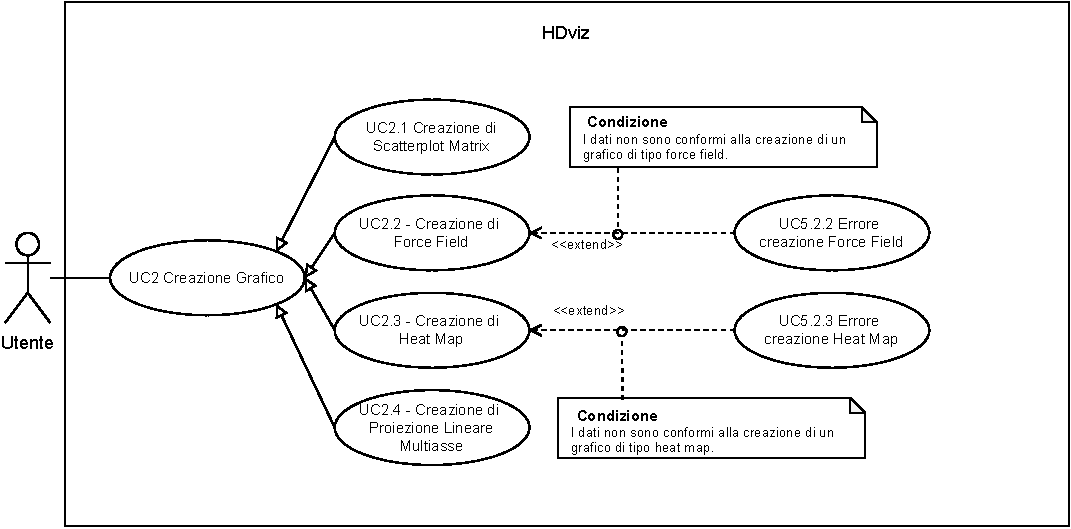
\includegraphics[width=0.8\textwidth]{componenti/casi-duso/diagrammi/UC2.pdf}
    \caption{Diagramma rappresentante UC2}
    \label{fig:UC2}
\end{figure}


\begin{itemize}
    \item \textbf{Descrizione}: L’utente vuole procedere con la fase di esplorazione
                                dati mediante la visualizzazione del dataset
                                attraverso uno dei diversi grafici proposti dall’applicativo
                                che ne costruisce uno e lo visualizza.
	
    \item \textbf{Attore primario}: Utente;
    
    \item \textbf{Precondizione}:   In HD Viz è stato caricato un dataset valido e
									l'utente ha aperto il menu di creazione di un grafico.

    \item \textbf{Postcondizione}:  Viene calcolato il grafico della tipologia scelta dall'utente dai dati 
									dal dataset corrente. 
									
									Viene inoltre mostrata la nuova visualizzazione all'utente.

	\item \textbf{Scenario principale}:
		\begin{enumerate}
			\item L'utente seleziona l'opzione che desidera tra le tipologie di grafico. \hyperref[ssub:uc2.1]{UC2.1}
			\item HD Viz visualizza il grafico ottenuto dalla costruzione della scelta dell'utente.
		\end{enumerate}
\end{itemize}

\subsubsection{UC2.1 - Selezione grafico}
\label{ssub:uc2.1}
\begin{itemize}

	\item \textbf{Descrizione}: L’utente seleziona la tipologia di grafico che desidera costruire.

    \item \textbf{Attore primario}: Utente.

	\item \textbf{Precondizione}:   Un dataset è stato correttamente importato. 
	
    \item \textbf{Postcondizione}:  Viene calcolato il grafico della tipologia selezionata dall'utente.

	\item \textbf{Generalizzazioni:}:  L'utente seleziona il grafico desiderato tra:

		\begin{enumerate}
			
			\item Selezione di Scatterplot matrix \hyperref[ssub:uc2.2]{UC2.2}
			\item Selezione di Force Field \hyperref[ssub:uc2.3]{UC2.3}
			\item Selezione di Heat Map \hyperref[ssub:uc2.4]{UC2.4}
			\item Selezione di Proiezione Lineare Multiasse \hyperref[ssub:uc2.5]{UC2.5}
			\item Selezione di Distance Map \hyperref[ssub:uc2.6]{UC2.6}
			
		\end{enumerate}

\end{itemize}


\subsubsection{UC2.2 - Selezione di Scatter Plot matrix}
\label{ssub:uc2.2}
\begin{itemize}

    \item \textbf{Attore primario}: Utente;

    \item \textbf{Precondizione}:   L'utente ha selezionato la voce \emph{Scatter Plot Matrix} dal menu di creazione di un grafico.

    \item \textbf{Postcondizione}:  Viene calcolato il grafico di tipo \emph{"Scatter Plot Matrix"}.

	\item \textbf{Scenario Principale}: HD Viz calcola uno \emph{Scatter Plot Matrix} dal dataset corrente.
\end{itemize}


\subsubsection{UC2.3 - Selezione di Force Field}
\label{ssub:uc2.3}
\begin{itemize}

    \item \textbf{Attore primario}: Utente;

    \item \textbf{Precondizione}:   L'utente ha selezionato la voce \emph{Force Field} dal menu di creazione di un grafico.

    \item \textbf{Postcondizione}:  Viene calcolato il grafico di tipo \emph{"Force Field"}.
	
	\item \textbf{Scenario Principale}: HD Viz calcola un \emph{Force Field} dal dataset corrente.

\end{itemize}


\subsubsection{UC2.4 - Selezione di Heat Map}
\label{ssub:uc2.4}
\begin{itemize}

    \item \textbf{Attore primario}: Utente;

	\item \textbf{Precondizione}:   L'utente ha selezionato la voce \emph{Heat Map} dal menu di creazione di un grafico.

    \item \textbf{Postcondizione}:  Viene calcolato il grafico di tipo \emph{"Heat Map"}.

	\item \textbf{Scenario Principale}: HD Viz calcola una \emph{Heat Map} dal dataset corrente.

\end{itemize}


\subsubsection{UC2.5 - Selezione di Proiezione Lineare Multi Asse}
\label{ssub:uc2.5}
\begin{itemize}

    \item \textbf{Attore primario}: Utente;

    \item \textbf{Precondizione}:   L'utente ha selezionato la voce \emph{Proiezione Lineare Multi Asse} dal menu di creazione di un grafico.

    \item \textbf{Postcondizione}:  Viene calcolato il grafico di tipo \emph{"Proiezione lineare multiasse"}.

	\item \textbf{Scenario Principale}: HD Viz calcola una \emph{Proiezione Lineare Multiasse} dal dataset corrente.
\end{itemize}

\subsubsection{UC2.6 - Selezione di Distance Map}
\label{ssub:UC2.6}
\begin{itemize}
	\item \textbf{Attore primario}:		Utente;
	\item \textbf{Precondizione}:		L'utente ha selezionato la voce \emph{Distance Map} dal menu di creazione di un grafico.
	\item \textbf{Postcondizione}:		Viene calcolato il grafico di tipo\emph{"Distance Map"}.
	\item \textbf{Scenario Principale}: HD Viz calcola una  \emph{Distance Map} dal dataset corrente.
\end{itemize}